\documentclass[UTF8]{ctexart}
\usepackage{hyperref}
\usepackage{abstract}
\usepackage[margin=1in]{geometry}
\usepackage{graphicx}
\begin{document}

\title{透镜焦距的测量}
\author{2019012137  物理92  张鸿琳}
\maketitle
\begin{abstract}
本实验主要围绕凹透镜与凸透镜的焦距测量展开。从透镜的基本成像规律出发,利用现实生活中的常用物品,从多种角度出发,测量透镜焦距,从而更好地理解了透镜成像的规律,掌握了简单光路的分析和调节技术,深刻地认识了焦距所代表的透镜改变光束的能力强弱的意义,为未来深入学习更复杂的光学系统打下了基础。



\centering
\textbf{Keywords:}凹透镜,凸透镜,焦距,成像
\end{abstract}

\newpage
\tableofcontents
\newpage
\section{实验仪器步骤与数据处理}
\subsection{薄凸透镜焦距的测量}
\subsubsection{实验仪器}
薄凸透镜,光屏,光源(小灯泡加透镜模拟的平行光源以及手机手电筒充当的点光源),平面镜,刻度尺。
\subsubsection{几种测量焦距的方法与数据处理}
\paragraph{相似三角形法}
\begin{itemize}
\item 将光屏,凸透镜,光源三个光学元件调节共轴;
\item 调节光屏距离,得到合适大小的像;
\item 测量凸透镜尺寸D,透镜和光屏距离S,像尺寸d;
\item 由相似三角形原理,得到焦距为$f=\frac{DS}{D-d}$。
\end{itemize}
由该方法,测得D=3.75cm,S=9.72cm,d=0.35cm,故而焦距f=10.72cm。
\paragraph{自准法}
\begin{itemize}
\item 将平面镜,凸透镜,点光源三个光学元件调节共轴;
\item 不断调节点光源与凸透镜间距离,直到点光源自身亮度与反射亮度叠加最大;
\item 测量此时点光源与凸透镜间距离,即为焦距。
\end{itemize}
由此方法,得到焦距为f=10.50cm。
\paragraph{物距像距法}
\begin{itemize}
\item 将光屏,凸透镜,小箭矢,光源四个光学元件调节共轴;
\item 固定箭矢,调节光屏位置,当箭矢的像在光屏上最清晰时,测量箭矢,透镜,像间的距离,即物距p,像距q,由公式$\frac{1}{f}=\frac{1}{p}+\frac{1}{q}$得到焦距,再调节箭矢位置,得到多组数据。
\end{itemize}
由此方法,测得原始数据见“原始测量数据”,经处理数据见下表,
\begin{table}[htbp!] 
\centering 
\begin{tabular}{|c|c|c|} 
\hline 
 物距p(cm) &  像距q(cm)&焦距f(cm)  \\ 
\hline 
16.82 & 26.51&10.29  \\ 
\hline 
14.51 & 32.68 &10.05\\ 
\hline 
26.74 & 17.42 &10.55\\ 
\hline
\end{tabular} 
\end{table}
故而焦距大约为f=10.30cm。
\paragraph{共轭法}
\begin{itemize}
\item 将光屏,凸透镜,小箭矢,光源四个光学元件调节共轴;
\item 首先找到一组距离为b的物与像,之后调节透镜位置,使像仍然保持在原来位置,测量此时透镜位置位移a,由公式$\frac{1}{f}=\frac{1}{p}+\frac{1}{q}$,得到焦距$f=\frac{b^2-a^2}{4b}$,调节初始物像距离b,在进行同样操作,得到多组数据。
\end{itemize}
对得到的数据进行处理,得到下表,可见焦距大约为f=10.23cm。
\begin{table}[htbp!] 
\centering 
\begin{tabular}{|c|c|c|} 
\hline 
 物像距离b(cm) &  透镜位置位移(cm)&焦距(cm)  \\ 
\hline 
65.71 & 40.02 &10.33\\ 
\hline 
60.39 & 34.61 &10.14\\ 
\hline 
55.66 & 28.72 &10.21 \\ 
\hline
\end{tabular} 
\end{table}
\paragraph{(其他方法)}由于其他方法的基本内涵已由上述方法概括,只是测量方式有所不同(如同样可以采用插针法记录光路,操作同下面测量凹透镜焦距实验),由于实验条件简陋,较难实现,故而不再赘述。
\subsubsection{误差分析}
\paragraph{影响因素}
\begin{itemize}
\item 由于透镜边缘打磨的问题,导致透过的光线发生较为明显的衍射,所以像点尺寸存在较大误差;
\item 光源并不是严格的平行光源或者点光源;
\item 由于光学元件本身的形状,故而在测量相对距离时有一定误差;
\item 在某些临界条件下,由于实验条件较为简陋,很难判定其具体位置,有较大误差。
\end{itemize}
\paragraph{为减小影响做出的努力}
\begin{itemize}
\item 测量相对距离时,从多个角度测量,取平均;
\item 在透镜边缘处添加遮挡物,从而减小由于打磨不够而边缘处衍射严重引起的误差;
\item 取合适的距离和环境,使得光源特性尽量符合实验要求的条件;
\item 判定临界条件时,不断变更元件位置,反复比较,尽量减小误判。
\end{itemize}
\subsection{薄凹透镜焦距的测量}
\subsubsection{实验仪器}
薄凹透镜,光屏,光源(小灯泡加透镜模拟的平行光源以及手机手电筒充当的点光源),刻度尺,针。
\subsubsection{几种测量焦距的方法与数据处理}
\paragraph{入射——出射法(插针法)}
\begin{itemize}
\item 将凹透镜固定,在凹透镜一侧平行于主轴插两根针 1、2;
\item 另一侧也插两根针 3、4,使得 3、4 针的像与 1、2 针共线,进而作出光路图,求得焦距。
\end{itemize}
由该方法,作图,测得凹透镜焦距约为f=7.51cm。
\paragraph{相似三角形法}
\begin{itemize}
\item 将光屏,凸透镜,光源三个光学元件调节共轴;
\item 调节光屏距离,得到合适大小的像;
\item 测量凸透镜尺寸d,透镜和光屏距离S,像尺寸D;
\item 由相似三角形原理,得到焦距为$f=\frac{dS}{D-d}$。
\end{itemize}
由该方法,测得d=2.80cm,D=5.21cm,S=6.53cm,故而f=7.58cm。
\paragraph{凹透镜放大率/视场法}
\begin{itemize}
\item 将凹透镜固定,其后放置一个刻度尺;
\item 调节刻度尺与透镜间距离,并从透镜另一侧沿凹透镜上边沿平视,记录距离S和可以看到的刻度D,多次调解相对位置,测得多组数据;
\item 测量凹透镜尺寸d,计算像距q,进而求得凹透镜焦距f。
\end{itemize}
测得的透镜直径为d=2.80cm,其他数据见“原始测量数据”,经过处理得到下表,可见焦距约为f=7.50cm。
\begin{table}[htbp!] 
\centering 
\begin{tabular}{|c|c|c|} 
\hline 
透镜与刻度尺距离S(cm) &  可见刻度D(cm) &焦距f(cm) \\ 
\hline 
15.50 & 4.28&7.53 \\ 
\hline 
10.23 & 3.31 &7.50\\ 
\hline 
5.76 & 2.48 &7.47 \\ 
\hline
\end{tabular} 
\end{table}
\paragraph{(其他方法)}由于其他方法的基本内涵已由上述方法概括,只是测量方式有所不同,由于实验条件简陋,较难实现,故而不再赘述。
\subsubsection{误差分析}
\paragraph{影响因素}
\begin{itemize}
\item 由于透镜边缘打磨的问题,导致透过的光线发生较为明显的衍射,所以像点尺寸存在较大误差;
\item 在插针法中,由于使用的透镜较小,针的尺度其实相对较大,使得位置判定误差较大;
\item 由于光学元件本身的形状,故而在测量相对距离时有一定误差;
\item 光源并不是严格的平行光源或者点光源;
\item 在视场法中,较难保持平视,受实验者自身判定影响较大。
\end{itemize}
\paragraph{为减小影响做出的努力}
\begin{itemize}
\item 测量相对距离时,从多个角度测量,取平均;
\item 在透镜边缘处添加遮挡物,从而减小由于打磨不够而边缘处衍射严重引起的误差;
\item 取合适的距离和环境,使得光源特性尽量符合实验要求的条件;
\item 在插针法中,将针上某一固定位置作为判定平行以及作图的标准;
\item 在视场法中,多次做自身校准,同时多次测量,舍弃明显不合理的数据。
\end{itemize}
\section{讨论}
本实验比较贴近于生活日常,用常见工具进行试验,有利于培养未来对于透镜现象的感性分析,但是也因为如此,使得试验精度很差,更进一步的数据处理难以展开,涉及的数理推导也较为简单,在这方面收获较小。不过收获最大的应该是误差分析方面,之后的实验条件有时也很难达到理想的精确度,这次对各种可见可感的误差的分析使得误差分析的经验增加了,增加了对误差来源的认识,故而以后考虑误差问题会更加全面。
\section{原始测量数据}
\subsection{“薄凸透镜焦距的测量”的原始数据}
利用物距像距法测量薄凸透镜焦距时测得的数据如下:
\begin{table}[htbp!] 
\centering 
\begin{tabular}{|c|c|} 
\hline 
 物距p(cm) &  像距q(cm) \\ 
\hline 
16.82 & 26.51  \\ 
\hline 
14.51 & 32.68 \\ 
\hline 
26.74 & 17.42 \\ 
\hline
\end{tabular} 
\end{table}

利用共轭法测量薄凸透镜焦距时测得的数据如下:
\begin{table}[htbp!] 
\centering 
\begin{tabular}{|c|c|} 
\hline 
 物像距离b(cm) &  透镜位置位移(cm)  \\ 
\hline 
65.71 & 40.02 \\ 
\hline 
60.39 & 34.61 \\ 
\hline 
55.66 & 28.72  \\ 
\hline
\end{tabular} 
\end{table}
\subsection{“薄凹透镜焦距的测量”的原始数据}
利用凹透镜放大率/视场法测量薄凹透镜焦距时测得的数据如下:
\begin{table}[htbp!] 
\centering 
\begin{tabular}{|c|c|} 
\hline 
透镜与刻度尺距离S(cm) &  可见刻度D(cm)  \\ 
\hline 
15.50 & 4.28 \\ 
\hline 
10.23 & 3.31 \\ 
\hline 
5.76 & 2.48  \\ 
\hline
\end{tabular} 
\end{table}
\subsection{测量实验装置照片}
\subsubsection{凸透镜焦距测量}
\paragraph{相似三角形法}
\begin{center} 
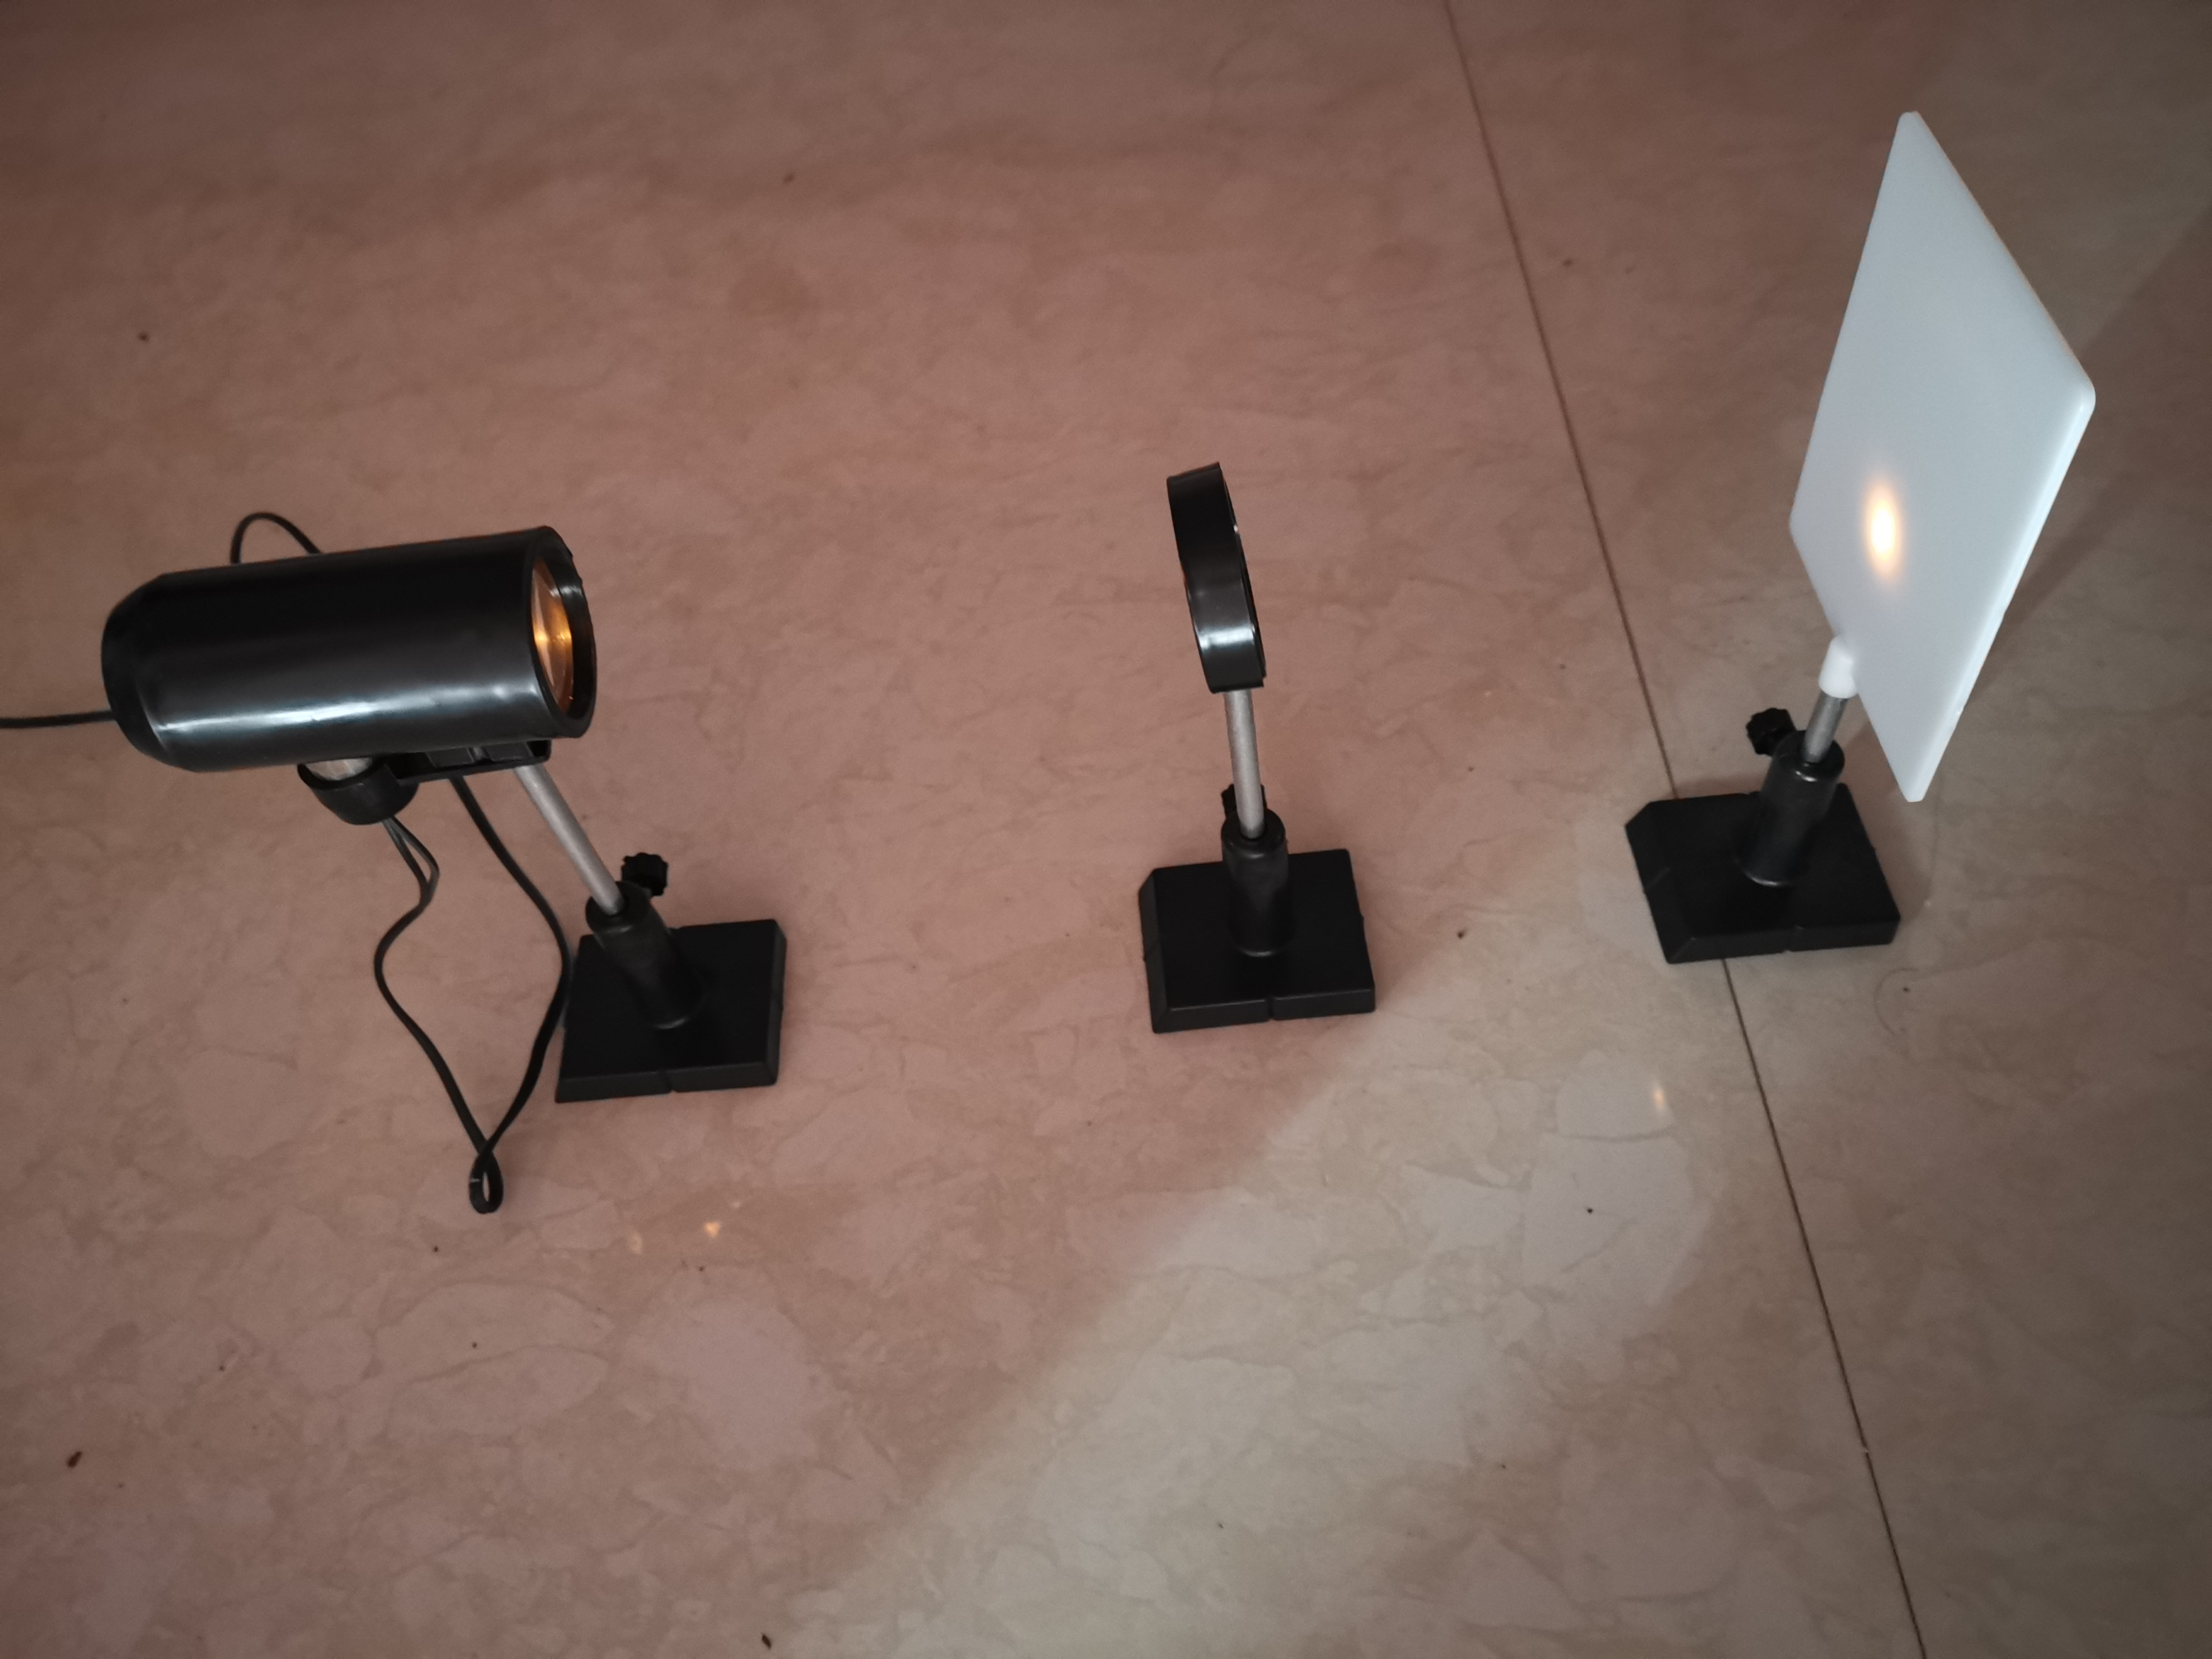
\includegraphics[width=0.95\textwidth]{A.jpg} 
\end{center}
\paragraph{物距像距法}
\begin{center} 
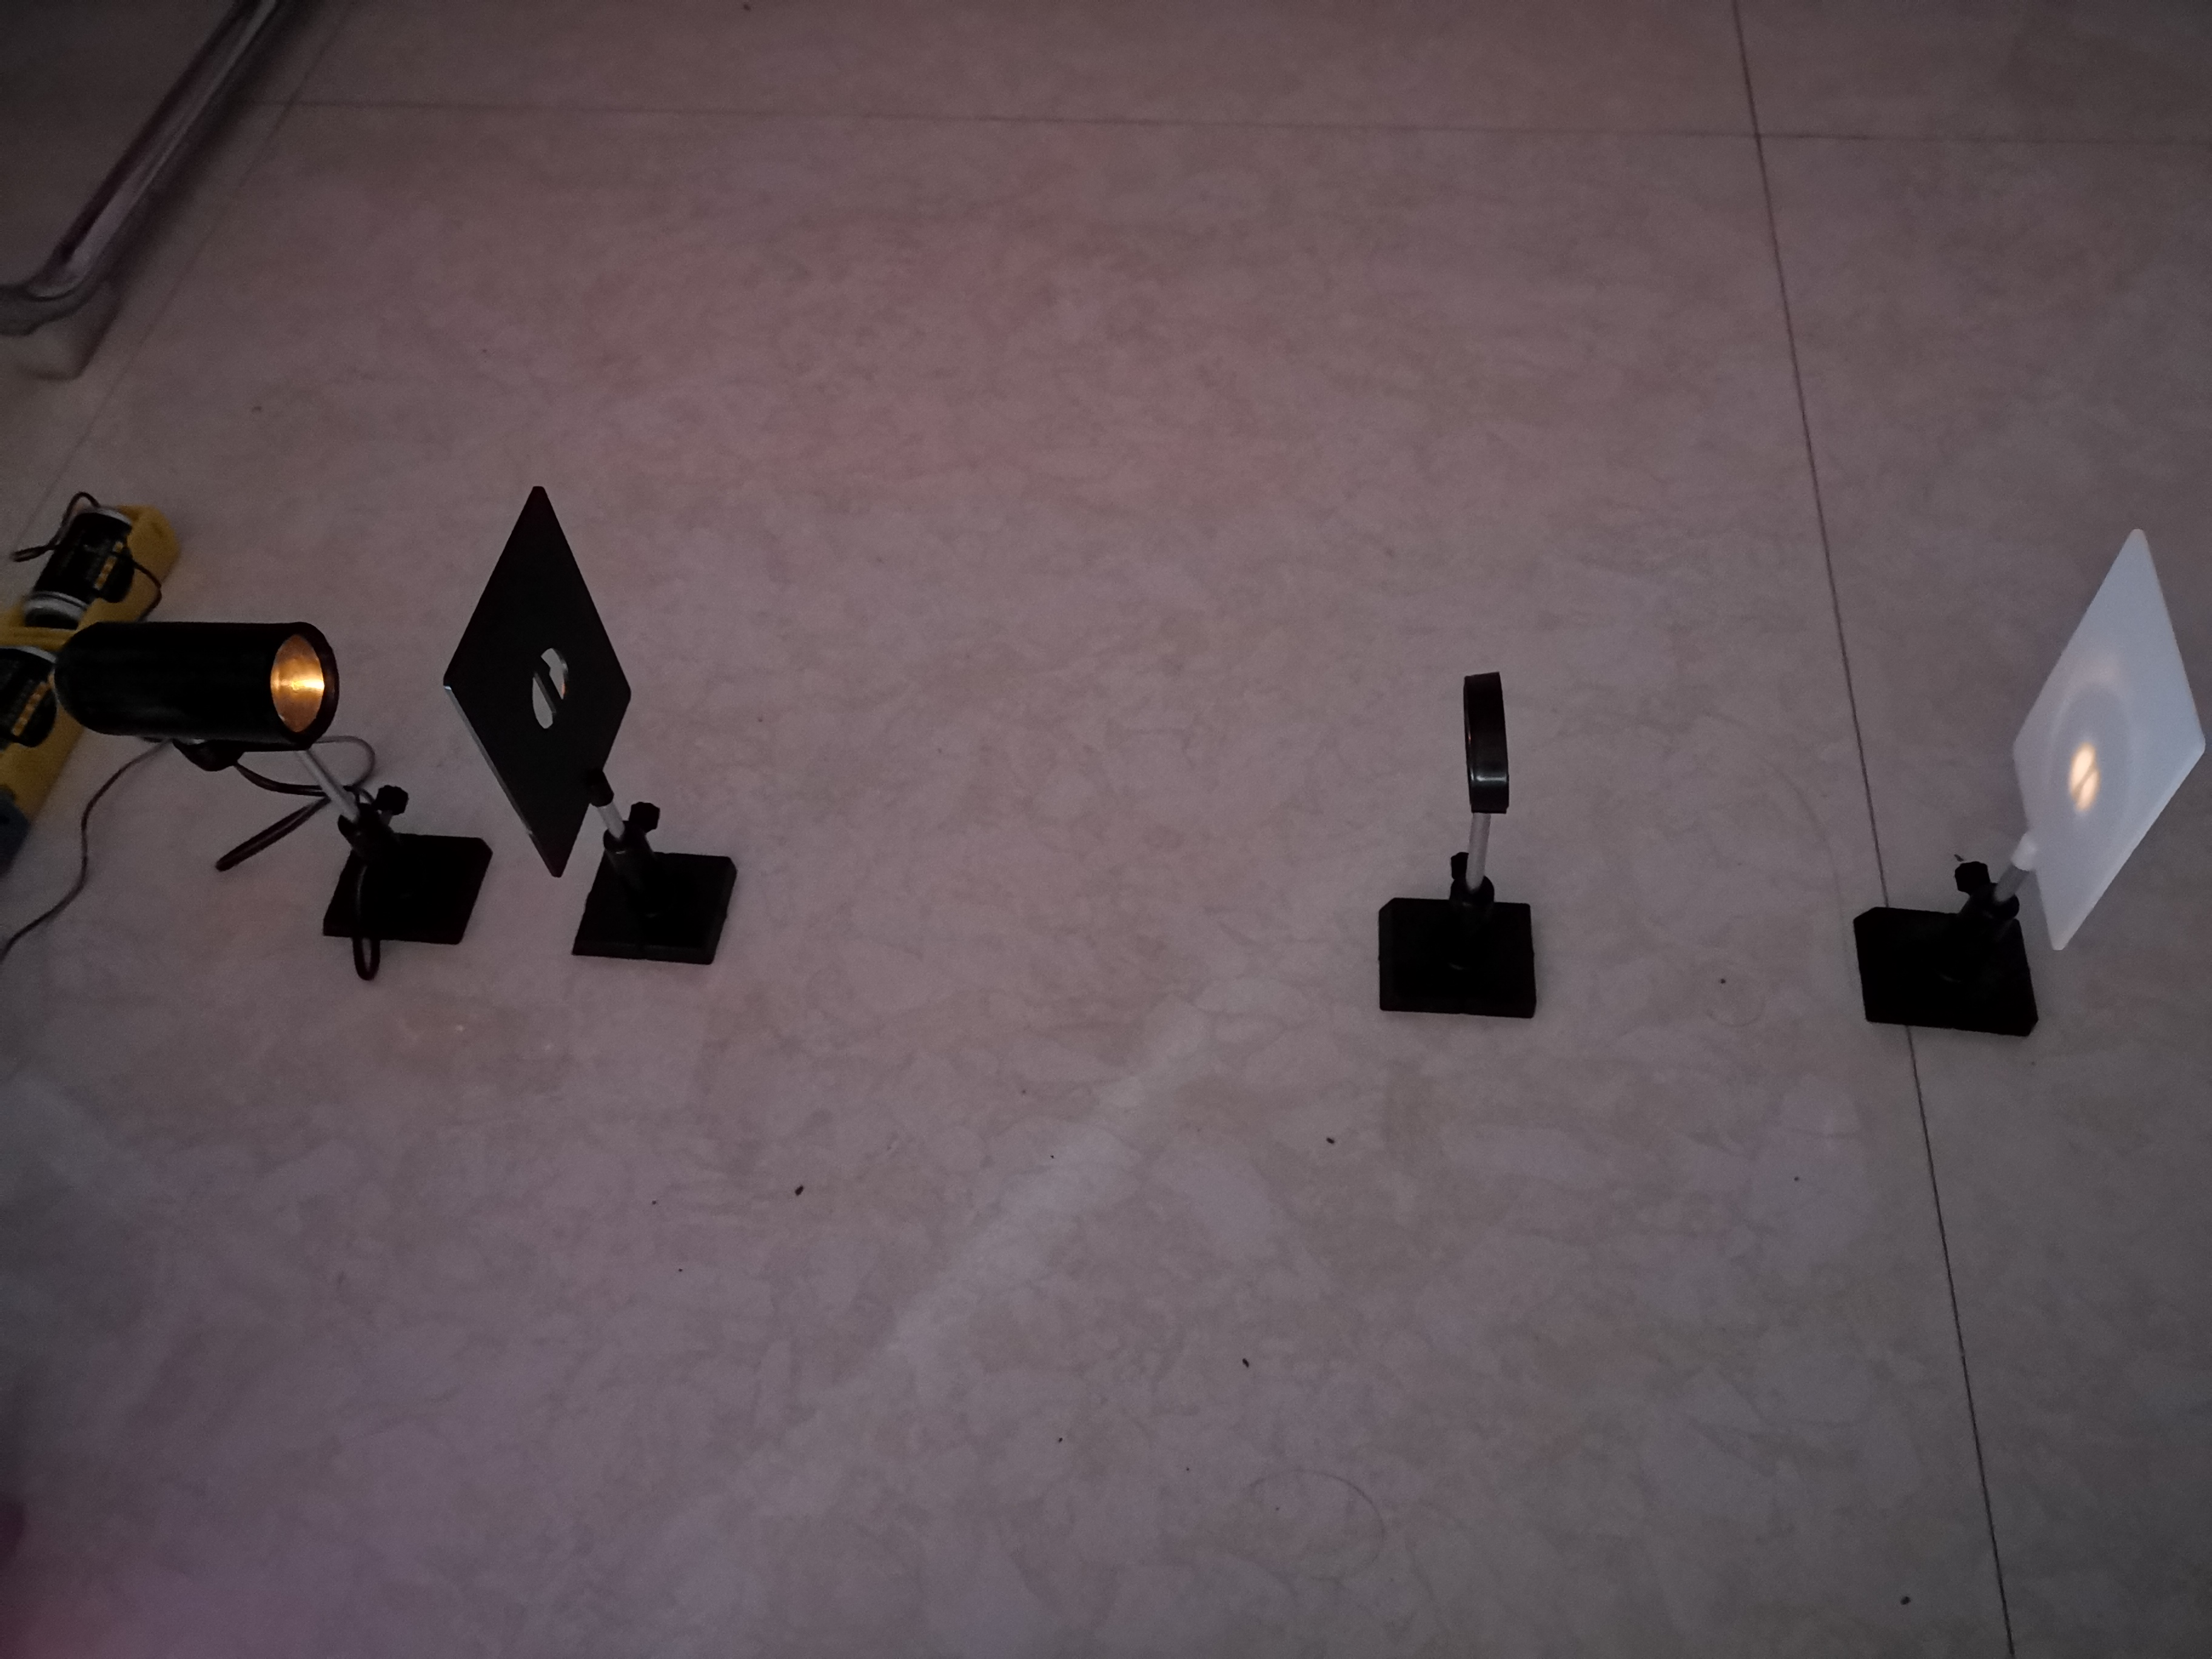
\includegraphics[width=0.95\textwidth]{B.jpg} 
\end{center}
\subsubsection{凹透镜焦距测量}
\paragraph{入射——出射法(插针法)}
\begin{center} 
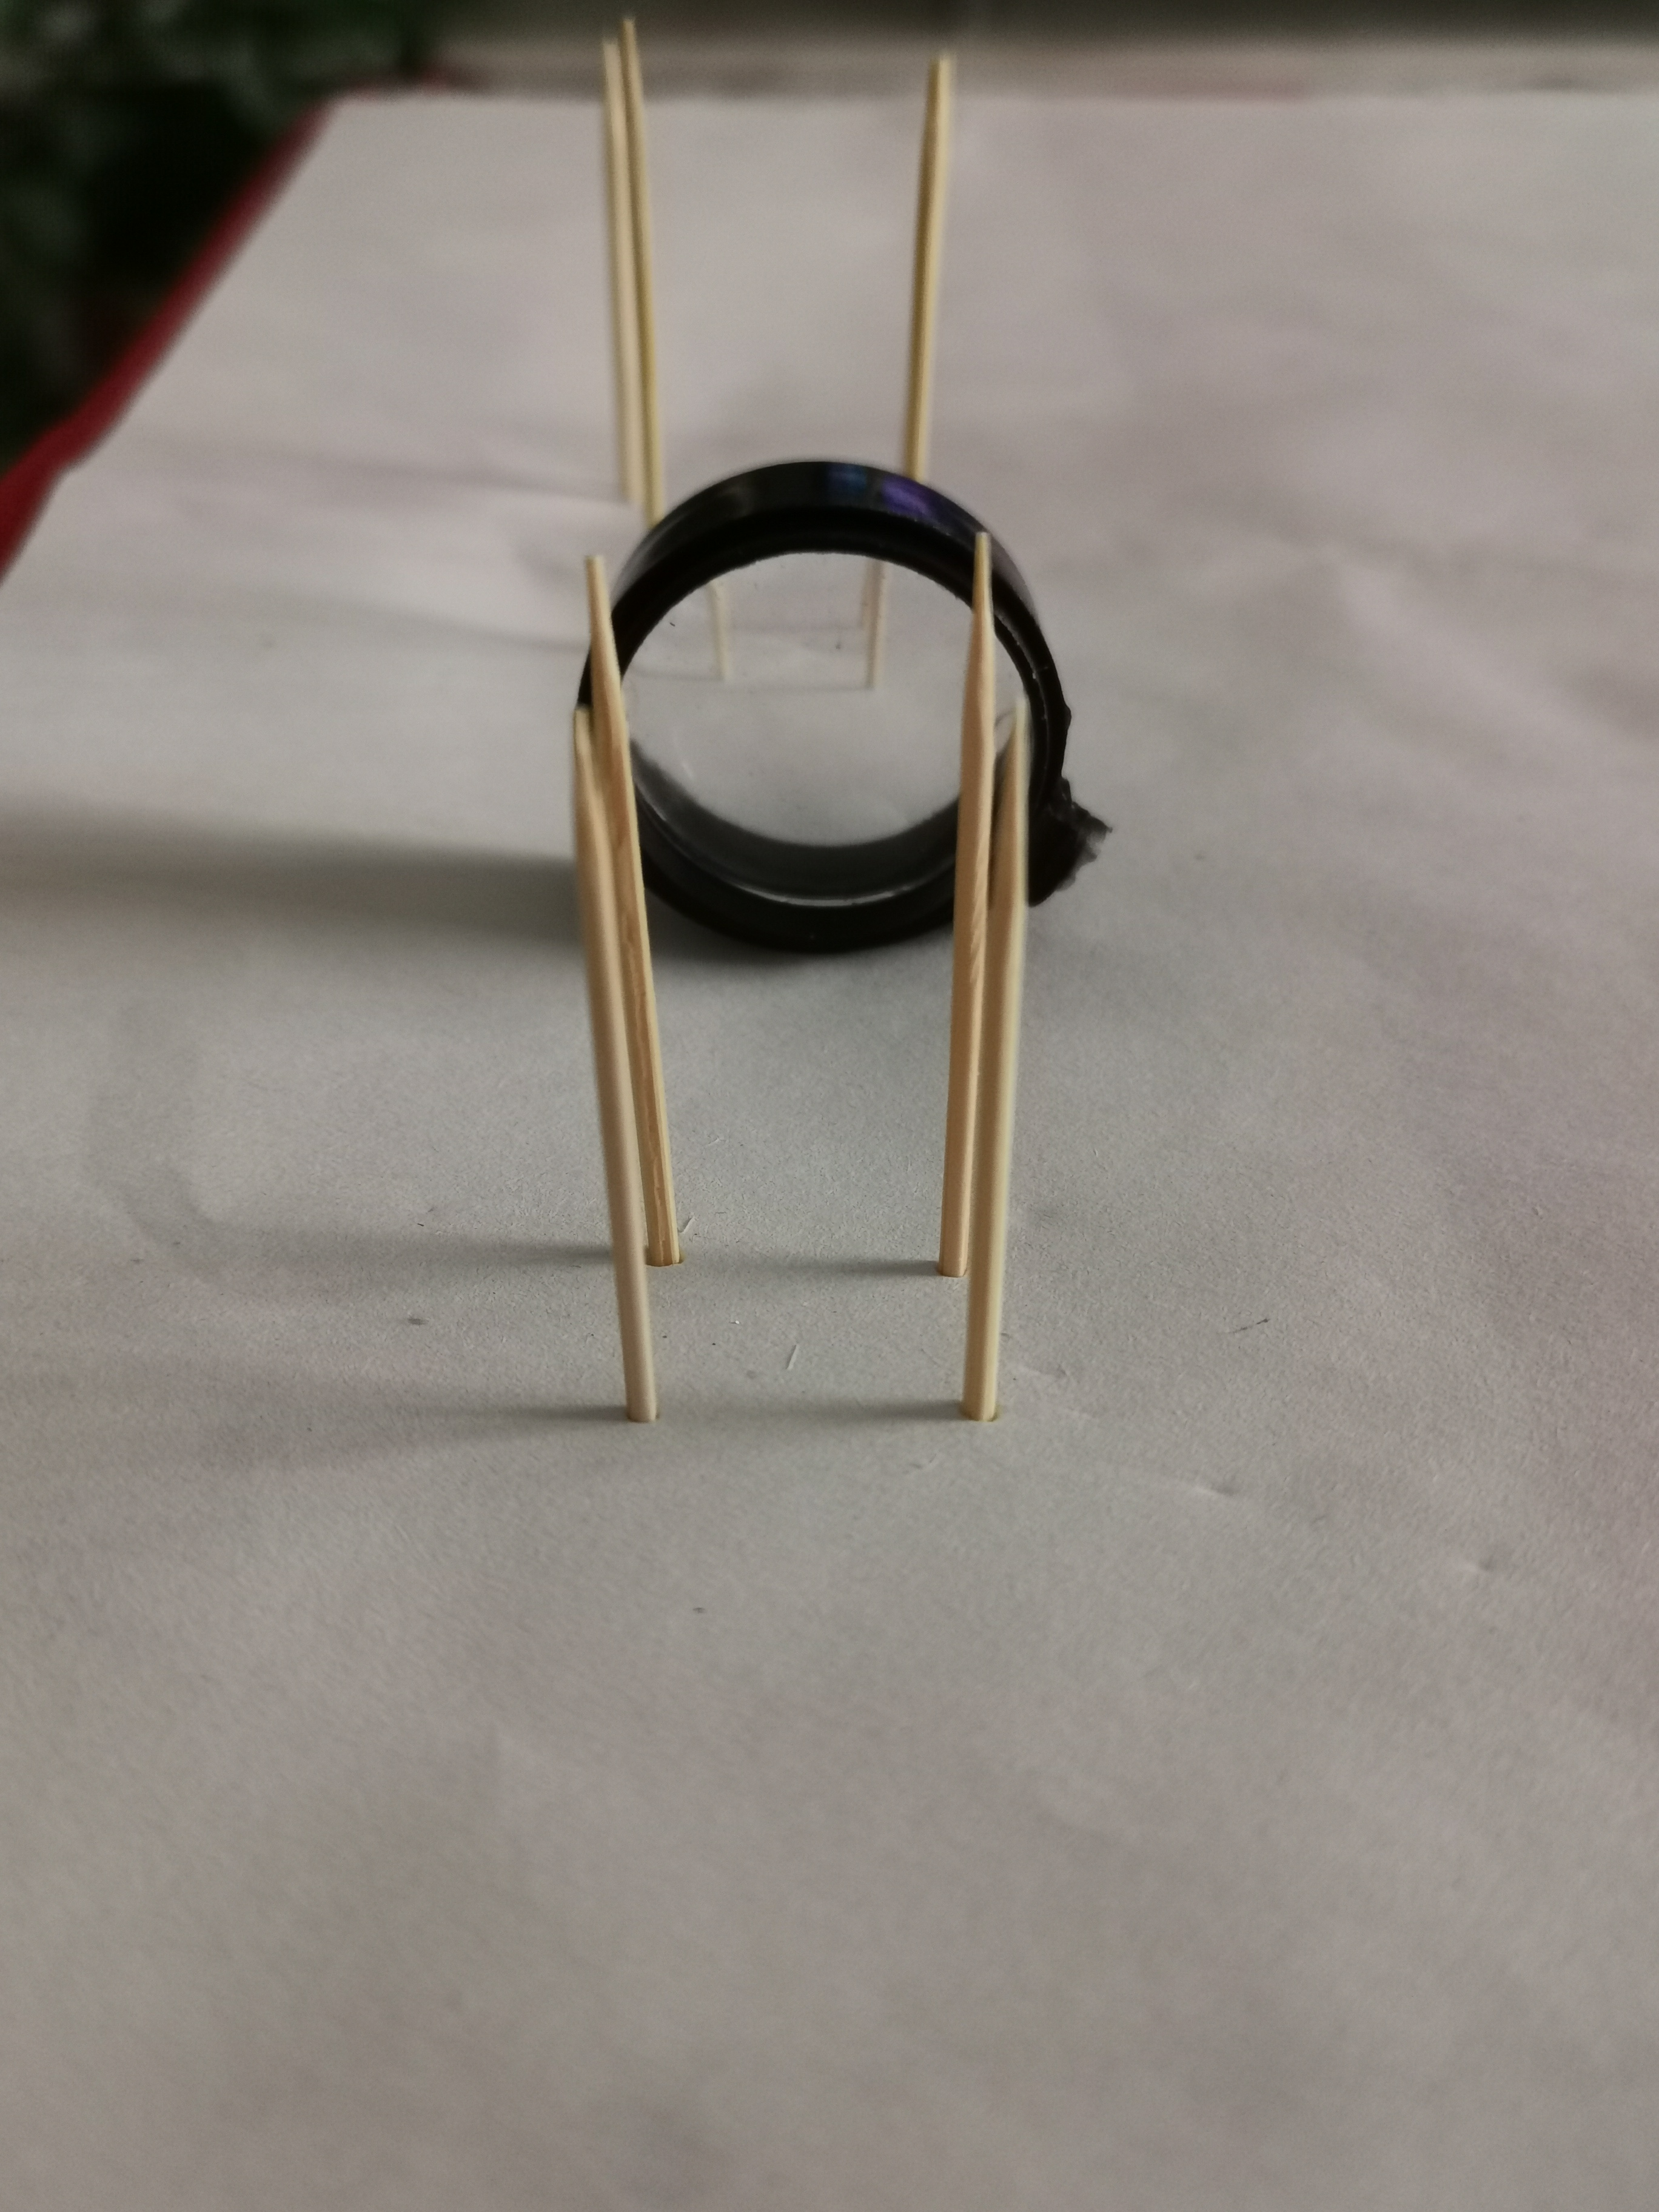
\includegraphics[width=0.95\textwidth]{C.jpg} 
\end{center}
\begin{thebibliography}{123456} 
\bibitem{ref1} 朱鹤年. 新概念基础物理实验讲义. 清华大学出版社. 2013. 
\bibitem{ref2} 王子余. 几何光学和光学设计. 浙江大学出版社.1989. 
\bibitem{ref3} 李晓彤. 几何光学和光学设计. 浙江大学出版社.1997. 
\bibitem{ref4} 叶韵.圆柱透镜成像规律探究. 物理教学.2020年2月.
\end{thebibliography}


\end{document}
